\subsection{5.3 RL 性能}\label{rl-performance}

训练过程中会监控性能变化，以验证扩展后的 RL 算力确实有效。如图 9 所示，
Flash 与 Pro 在 RL 训练中于 DeepSWE v1.1、AutomationBench v1.0.6 和 MiMo
Visual Coding 上均取得整体提升，尽管不同 checkpoint 之间存在波动。这些提升
通常伴随总 token 数的增长，说明更强的任务表现与更大的 token 使用量同步出现。
我们进一步考察多脚手架训练的效果，结果见图 10。该专项训练在四个训练用
mini-harness 以及三个留出脚手架：codex、claude code 和 mini-swe-agent 上，
都提升了 DeepSWE v1.1 的表现。尽管 checkpoint 之间有波动，三个留出脚手架在
训练过程中均持续改善，其平均 Pass@1 从约 50\% 提升到 66\%。训练脚手架与
留出脚手架之间的平均表现差距也同时收窄，说明学到的编码能力可以跨脚手架
实现迁移。这些结果支持我们使用轻量、模块化的 mini-harness 在 RL 中引入
可控多样性的设计。




\begin{figure}[htbp]
\centering

\includegraphics[width=\linewidth]{images_hi/fig10.png}
\caption{多脚手架训练过程中 DeepSWE v1.1 上的 Pass@1，分别用（a）训练脚手架和（b）留出脚手架评估。较浅的曲线为各脚手架单独的结果；粗橙色曲线为每个面板内的均值。}
\label{fig:10}
\end{figure}


\subsection{5.4 冻结路由器以稳定 RL}\label{router-freezing-for-stable-rl}

图 11 对比了两次仅 MoE 路由器是否冻结不同的 MiMo-V2.6-Pro RL 运行，追踪
解码器第 9 层的三项专家负载统计量：变异系数（CV）、峰值负载因子
（max/mean），以及负载低于均值 0.1$\times$ 的冷专家占比（负载按步归一化）。
当路由器可训练时，我们观察到严重的负载坍缩问题：三项指标在前 20 步内均
单调上升，CV 从 0.78 升至 2.0，峰值负载从 6$\times$ 升至 16$\times$，冷专家
占比从 0.5\% 升至 22\%。为定位原因，我们把第 20 步 checkpoint 的路由器参数
恢复到 RL 前的初始值，其余参数保持不变：负载均衡恢复到接近初始水平，而
基准表现不变，说明坍缩由路由器漂移驱动，而非专家权重退化。因此我们在 RL
训练中冻结路由器；冻结路由器的运行中三项统计量保持平稳（CV $\approx$ 0.7，
峰值负载 $\approx$ 5.5$\times$，冷专家占比接近 1\%），基准表现正常增长。

\subsection{5.5 RL 失败分析}\label{rl-failure-analysis}

图 12 汇总了 MiMo-V2.6-Pro 与 MiMo-V2.6-Flash 训练运行中的中断情况。基础
设施故障主要是 GPU 显存双比特错误（DBE）。Flash 还曾在 Kubernetes 故障
导致 Cyber 任务集群中的 pod 在第 15 与第 16 步之间崩溃后重启。Pro 在第 14 步
之后评分器网络不可达而重启。rollout 故障出现在部分 rollout 设置中：启动后
较短的 rollout 先完成，使 Predictive Rollout Dispatch（§6.3）中的长度估计
产生偏差，并耗尽 GPU 与 pinned 主机内存的 KV 池。尽管早期已做改进，某个
脚手架后来在同一代码数据集上产生的 rollout 长度不到其他脚手架的一半，使
重启后第二、三步的估计发生偏移。训练故障是由 micro-batch 内 MoE 不均衡
导致的 GPU 显存不足（OOM）：在某一层，一个专家并行（EP）rank 收到的 token
负载超过均值的 30$\times$，而整个 batch 的负载相对均衡。我们调整并行方式以
减少激活内存并容纳这些峰值。驱动故障出现在 Flash 后期的 packing 阶段，因为
更长的序列使每节点数据量超过主机内存容量。虽然 packing 已跨节点分布
（§6.2），本地内存需求仍导致 CPU OOM 并中断了运行。





\begin{figure}[htbp]
\centering

\includegraphics[width=\linewidth]{images_hi/fig11.png}
\caption{MiMo-V2.6-Pro 在 RL 过程中解码器第 9 层（384 个专家）的专家负载均衡情况，对比冻结路由器与不冻结路由器的运行。(a) 专家负载的变异系数。(b) 峰值负载因子（max/mean）。(c) 负载低于均值 0.1$\times$ 的冷专家占比。}
\label{fig:11}
\end{figure}


\begin{figure}[htbp]
\centering

\includegraphics[width=\linewidth]{images_hi/fig12.png}
\caption{MiMo-V2.6-Pro 与 MiMo-V2.6-Flash 在 30 个训练步上的时间线，按经过时间对齐。浅橙色表示已完成的步；其他颜色按原因表示失败与恢复区间。}
\label{fig:12}
\end{figure}


\subsection{5.6 通过 MOPD2 扩展能力}\label{broadening-capabilities-via-mopd2}

混合 RL 之后，我们用多前缀多教师同策略蒸馏（MOPD2）来整合针对不同任务
训练的教师能力，其中包括难以验证的任务。在 MiMo-V2-Flash 的 MOPD
（Core Team et al., 2026; Ma et al., 2026）基础上，我们在有合适 mixRL 教师的
领域保留学生自主 rollout（标准 MOPD），并加入前缀条件的单轮 rollout
（Liao et al., 2026）。图 13 展示了教师配置以及标准和前缀条件两种蒸馏流程。





\begin{figure}[htbp]
\centering
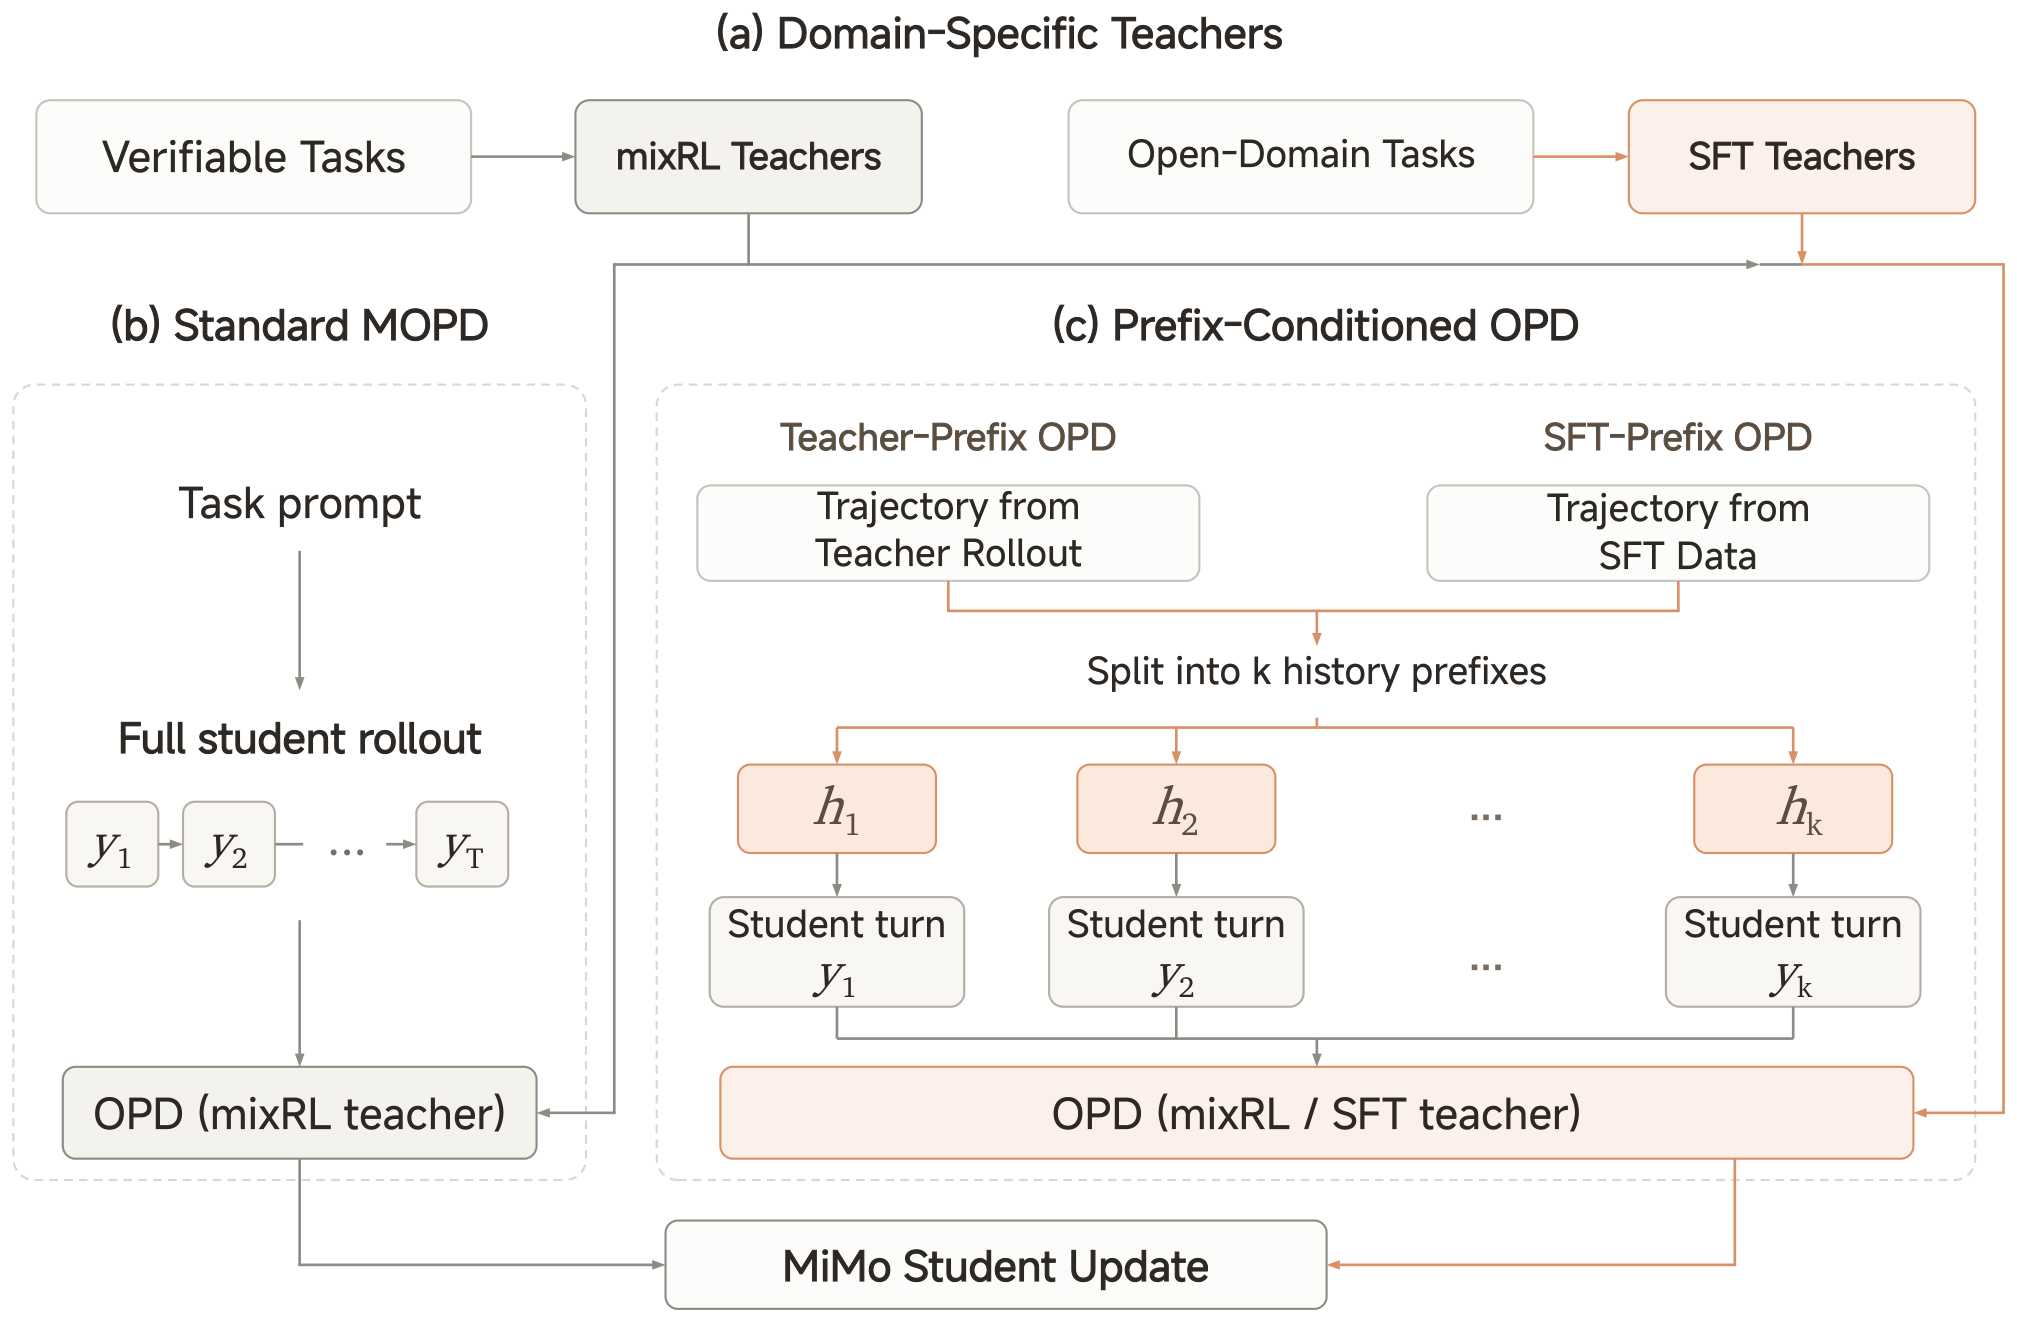
\includegraphics[width=\linewidth]{images_hi/fig13.png}
\caption{MiMo MOPD2 概览。(a) 领域专用教师在可验证任务上用 MixRL 训练，或在开放域任务上用合成演示做 SFT。(b) 标准 MOPD 用 RL 教师监督学生的完整 rollout。(c) 前缀条件 OPD 复用教师 rollout（Teacher-Prefix OPD）或 SFT 数据（SFT-Prefix OPD）中的轨迹。一条含 $k$ 个助手轮次决策点的源轨迹可得到 $k$ 个完整历史前缀 \(h _ { i } ,\)，每个前缀都可初始化一个单独由学生生成的轮次 \(y _ { i }\)，供相应领域教师做 token 级蒸馏。SFT 数据提供的是前缀上下文，而非固定的续写目标。}
\label{fig:13}
\end{figure}

前缀来自教师 rollout（Teacher-Prefix OPD）或 SFT 数据（SFT-Prefix OPD）。
一条含 $k$ 个助手轮次的轨迹提供 $k$ 个完整历史前缀，每个前缀在对应轮次之前
结束。学生从每个前缀采样一个新轮次，不重新生成此前的交互。预先指定的教师
以相同历史和学生的前序 token 为条件提供 token 级监督。

对于难以设计可靠 RL 奖励的开放域任务，我们用高质量合成演示训练 SFT 教师。
这类训练对长时程任务中学生反复偏离后所到达的历史覆盖可能有限
（Xu et al., 2025）。因此 SFT-Prefix OPD 让每次 rollout 都从固定的演示前缀
开始，限制采样轮次之前的偏离。演示提供上下文，学生则生成自己的续写，而不是
模仿固定回答。

MOPD2 进一步把 RL 训练模型的能力扩展到难以进行可靠训练时验证的领域，包括
环境复杂或校验器难以设计的领域，例如长时程游戏开发、科学研究和具身智能。
MiMo-V2.6 的最终评测结果见表 3。MiMo-V2.6 系列相对 MiMo-V2.5 有大幅提升，
在多个领域达到与前沿模型相当的表现。



表 3 MiMo-V2.6 与上一代模型及前沿模型在智能体基准上的对比。

{\footnotesize\setlength{\tabcolsep}{3pt}\def\LTcaptype{none} % do not increment counter
\begin{longtable}[]{@{}|L{13em}|C{7em}|C{7em}|C{7em}|C{7em}|C{7em}|C{7em}|@{}}
\toprule\noalign{}
\endhead
\bottomrule\noalign{}
\endlastfoot
\hline
基准 & MiMo-V2.6 Pro & MiMo-V2.6 Flash & MiMo-V2.5 Pro & Claude
Opus 5 & GPT-5.6 Sol & Claude Fable 5 \\
\hline
\multicolumn{7}{@{}l@{}}{%
代码智能体} \\
\hline
DeepSWE v1.1 & 71.9 & 67.9 & 19.0 & 74.0 & 73.0 & 70.0 \\
\hline
ProgramBench & 26.5 & 26.0 & 12.5 & 37.0 & 25.0 & 33.0 \\
\hline
MiMo Code Bench & 63.2 & 61.2 & 40.4 & 68.6 & 59.3 & - \\
\hline
\multicolumn{7}{@{}l@{}}{%
通用智能体} \\
\hline
AutomationBench v1.0.6 & 53.1 & 52.3 & 16.0 & 50.3 & 45.8 & 46.2 \\
\hline
Toolathlon-Verified & 76.9 & 73.6 & 49.1 & 80.6 & 74.9 & 77.9 \\
\hline
GDPval-AA 2.1 & 1673 & - & 1107 & 1708 & 1588 & 1595 \\
\hline
Agents\textquotesingle{} Last Exam & 31.6 & 27.6 & 13.2 & 31.6 & 30.8 &
25.7 \\
\hline
Terminal Bench 4.0 & 34.9 & 28.8 & 1.5 & 49.0 & 39.9 & 42.4 \\
\hline
Terminal Bench 2.1 & 89.9 & 87.6 & 65.2 & 89.1 & 88.8 & 84.3 \\
\hline
OSWorld-Verified & 82.0 & 80.8 & - & 83.4 & 83.0 & 86.0 \\
\hline
JobBench & 62.0 & 61.2 & 25.0 & 65.7 & 45.4 & 57.4 \\
\hline
\multicolumn{7}{@{}l@{}}{%
网络安全} \\
\hline
CyberGym & 94.0 & 95.1 & 40.0 & - & - & - \\
\hline
MiMo Cyber Bench & 80.2 & 77.2 & 0.0 & - & - & - \\
\hline
ExploitGym & 17.8 & 6.0 & 0.2 & 22.1 & 30.3 & 28.4 \\
\hline
ExploitBench & 47.9 & 25.3 & 16.6 & 70.0 & 78.5 & 78.0 \\
\hline
SEC Bench Pro & 66.3 & 47.5 & 17.7 & - & 79.1 & - \\
\hline
\multicolumn{7}{@{}l@{}}{%
视觉智能体} \\
\hline
MiMo Visual Coding & 72.3 & 71.5 & - & 70.0 & 73.4 & 69.1 \\
\hline
\end{longtable}
}
